% =====================================================================
%  PRESENTACION-WIDROW-LEHR.TEX
%  30 Años de Redes Neuronales Adaptativas: Perceptrón, Madaline y
%  Backpropagation (Widrow & Lehr, 1990).
%  Magíster en Ingeniería Informática USACH — Inteligencia Computacional 2026-1.
%
%  Estilo (colores, tema, márgenes, índice, portada) tomado de
%  example-presentation.tex (plantilla USACH).
%
%  Compilación:  pdflatex presentacion-widrow-lehr.tex   (x2)
% =====================================================================

\documentclass[aspectratio=169, 11pt, xcolor={dvipsnames,table}]{beamer}

% ── Paquetes base ────────────────────────────────────────────────────
\usepackage[utf8]{inputenc}
\usepackage[T1]{fontenc}
% Usa 'spanish' si la distribución lo tiene (tu equipo); si no, cae a 'english'
% para poder compilar igual en entornos sin babel-spanish. El contenido no cambia.
\IfFileExists{spanish.ldf}{%
  \usepackage[spanish, es-tabla, es-noshorthands]{babel}%
}{%
  \usepackage[english]{babel}%
}
\IfFileExists{lmodern.sty}{\usepackage{lmodern}\usepackage{microtype}}{}
\usepackage{amsmath, amssymb, mathtools, bm}
\usepackage{graphicx}
\usepackage{booktabs, array, multirow}
\usepackage{multicol}
\usepackage{caption}
\captionsetup{font=footnotesize, labelfont=bf}
\usepackage{tcolorbox}
\tcbuselibrary{skins}
\usepackage{tikz}
\usetikzlibrary{positioning, arrows.meta, calc, shapes.geometric, fit, backgrounds}
\hypersetup{hidelinks}
\usepackage{xcolor}

% ── Paleta USACH ─────────────────────────────────────────────────────
\definecolor{UsachAzul}{RGB}{7,27,73}
\definecolor{UsachNaranja}{RGB}{221,121,0}
\definecolor{UsachGris}{RGB}{57,64,73}
\definecolor{UsachGrisClaro}{RGB}{230,230,230}

% ── Theme + colores Beamer ───────────────────────────────────────────
\usetheme{Madrid}
\useinnertheme{rectangles}
\useoutertheme{infolines}
\setbeamertemplate{headline}{}
\setbeamertemplate{navigation symbols}{}

% - Reducir espacio entre bloques para aprovechar mejor la diapositiva -
\setlength{\medskipamount}{3pt plus 1pt minus 1pt}

% - AUTO-SHRINK MODERADO + MARGEN INFERIOR ---------
\makeatletter
\let\beamer@@frameORIG\beamer@@frame
\def\beamer@@frame[#1]{\beamer@@frameORIG[shrink=55,#1]}
\makeatother

% - FOOTLINE COMPACTA -----------------
\setbeamertemplate{footline}{%
  \leavevmode%
  \hbox{%
  \begin{beamercolorbox}[wd=.32\paperwidth,ht=2.25ex,dp=1ex,center]{author in head/foot}%
    \usebeamerfont{author in head/foot}\insertshortauthor
  \end{beamercolorbox}%
  \begin{beamercolorbox}[wd=.36\paperwidth,ht=2.25ex,dp=1ex,center]{title in head/foot}%
    \usebeamerfont{title in head/foot}\insertshorttitle
  \end{beamercolorbox}%
  \begin{beamercolorbox}[wd=.32\paperwidth,ht=2.25ex,dp=1ex,right]{date in head/foot}%
    \usebeamerfont{date in head/foot}\insertshortdate{}\hspace*{1.2em}%
    \insertframenumber{} / \inserttotalframenumber\hspace*{1.2ex}%
  \end{beamercolorbox}}%
  \vskip0pt%
}

\setbeamercolor{structure}{fg=UsachAzul}
\setbeamercolor{palette primary}{bg=UsachAzul, fg=white}
\setbeamercolor{palette secondary}{bg=UsachAzul!80, fg=white}
\setbeamercolor{palette tertiary}{bg=UsachAzul, fg=white}
\setbeamercolor{title}{fg=UsachAzul, bg=white}
\setbeamercolor{frametitle}{fg=white, bg=UsachAzul}
\setbeamercolor{section in head/foot}{bg=UsachAzul, fg=white}
\setbeamercolor{subsection in head/foot}{bg=UsachAzul!80, fg=white}
\setbeamercolor{author in head/foot}{bg=UsachAzul, fg=white}
\setbeamercolor{title in head/foot}{bg=UsachAzul!85, fg=white}
\setbeamercolor{date in head/foot}{bg=UsachAzul, fg=white}
\setbeamercolor{itemize item}{fg=UsachNaranja}
\setbeamercolor{itemize subitem}{fg=UsachNaranja!80}
\setbeamercolor{enumerate item}{fg=UsachNaranja}
\setbeamercolor{block title}{bg=UsachAzul, fg=white}
\setbeamercolor{block body}{bg=UsachAzul!5, fg=black}
\setbeamercolor{block title alerted}{bg=UsachNaranja, fg=white}
\setbeamercolor{block body alerted}{bg=UsachNaranja!8, fg=black}
\setbeamercolor{block title example}{bg=UsachGris, fg=white}
\setbeamercolor{block body example}{bg=UsachGris!8, fg=black}
\setbeamercovered{transparent=25}
\usefonttheme[onlymath]{serif}

\newcommand{\azul}[1]{\textcolor{UsachAzul}{#1}}
\newcommand{\naranja}[1]{\textcolor{UsachNaranja}{#1}}
\newcommand{\gris}[1]{\textcolor{UsachGris}{#1}}

% ── Cajas destacadas ─────────────────────────────────────────────────
\newtcolorbox{ideaclave}[1][]{
  colback=UsachNaranja!8, colframe=UsachNaranja!80!black,
  fonttitle=\bfseries, title=Idea clave, #1
}
\newtcolorbox{tipbox}[1][]{
  colback=green!5!white, colframe=green!50!black,
  fonttitle=\bfseries, title=Nota, #1
}

% ── Estilos TikZ (Adaline / taxonomía) ───────────────────────────────
\tikzset{%
  nodo/.style     ={circle, draw=UsachAzul!70, line width=0.7pt,
                    minimum size=16pt, inner sep=0pt, font=\scriptsize},
  suma/.style     ={circle, draw=UsachAzul!80, fill=UsachAzul!8,
                    line width=0.8pt, minimum size=20pt, font=\small},
  cuant/.style    ={rectangle, draw=UsachAzul!80, fill=UsachGrisClaro,
                    line width=0.8pt, minimum width=13pt, minimum height=18pt},
  peso/.style     ={circle, draw=UsachNaranja!80, fill=UsachNaranja!12,
                    minimum size=12pt, inner sep=0pt, font=\tiny},
  flarr/.style    ={-{Stealth[length=4pt]}, line width=0.6pt, draw=black!70},
  cat/.style      ={draw, rounded corners, fill=UsachAzul!10, align=center,
                    inner sep=4pt, font=\small\bfseries},
  arch/.style     ={draw, align=center, inner sep=3pt, font=\footnotesize},
  act/.style      ={align=center, font=\footnotesize\itshape},
  alg/.style      ={draw, rounded corners, fill=UsachNaranja!12, align=center,
                    inner sep=3pt, font=\footnotesize\bfseries},
  ln/.style       ={-, draw=black!65}
}

% ── Metadatos ────────────────────────────────────────────────────────
\title[Redes Neuronales Adaptativas: Perceptron, Madaline, Backprop]{%
  \textbf{30 Años de Redes Neuronales Adaptativas}}
\subtitle{Perceptrón, Madaline y Backpropagation \;(\textmd{Widrow \& Lehr, 1990})}
\author[I. Fernández G.]{%
  Iván Fernández G.}
\institute[USACH]{%
  \footnotesize Magíster en Ingeniería Informática - Universidad de Santiago de Chile\\
  Inteligencia Computacional 2026-1 \quad\textbar\quad Prof.\ Gonzalo Acuña Leiva}
\date{Julio 2026}

% =====================================================================
\begin{document}
% =====================================================================

% ─── PORTADA ─────────────────────────────────────────────────────────
{
\setbeamertemplate{background}{%
  \begin{tikzpicture}[remember picture, overlay]
    \fill[UsachAzul]
      (current page.north west) rectangle
      ([yshift=-1.6cm]current page.north east);
    \fill[UsachNaranja]
      ([yshift=-1.6cm]current page.north west) rectangle
      ([yshift=-1.75cm]current page.north east);
    \fill[UsachGris]
      ([yshift=0.55cm]current page.south west) rectangle
      ([yshift=0.65cm]current page.south east);
    \node[anchor=north west, xshift=8mm, yshift=-6mm,
          font=\bfseries\Large, text=white]
      at (current page.north west) {USACH};
    \node[anchor=north east, xshift=-8mm, yshift=-6mm,
          font=\footnotesize, text=white, align=right]
      at (current page.north east)
      {Magíster en Ingeniería Informática \;\textbullet\; Inteligencia Computacional 2026-1};
  \end{tikzpicture}}
\setbeamertemplate{footline}{}
\begin{frame}[plain,noframenumbering]
  \vspace*{1.2cm}
  \titlepage
\end{frame}
}

% ─── CONTENIDO GLOBAL ────────────────────────────────────────────────
\begin{frame}{Contenido}
\begin{columns}[t]
\column{0.5\textwidth}
\tableofcontents[sections={1-3}]
\column{0.5\textwidth}
\tableofcontents[sections={4-5}]
\end{columns}
\end{frame}

% Sin diapositivas divisorias entre secciones (versión condensada 10 min)
\AtBeginSection[]{}

% =====================================================================
\section{Introducción e historia}
% =====================================================================
\subsection{Motivación y línea histórica}

\begin{frame}{Contexto y línea histórica (1960--1990)}
\begin{block}{¿Qué aborda el artículo?}
Una \textbf{revisión} de 30 años de reglas de aprendizaje supervisado para redes
\emph{feedforward}: cómo \azul{adaptar los pesos} de elementos simples para clasificar o
hacer regresión a partir de ejemplos, con \naranja{generalización} a patrones no vistos.
\end{block}
\begin{columns}[T]
\column{0.6\textwidth}
\begin{itemize}\footnotesize
  \item \textbf{1960} - \azul{LMS} (Widrow \& Hoff) y regla del \azul{Perceptrón} (Rosenblatt), independientes.
  \item \textbf{Mediados 60s} - \azul{Madaline I} (MRI): primera red en capas entrenable.
  \item \textbf{1971--86} - \azul{Backpropagation} (Werbos; popularizada por Rumelhart, Hinton \& Williams).
  \item \textbf{1987--88} - \azul{MRII} y \azul{MRIII} (Andes): esta última, \textbf{equivalente a backprop}.
\end{itemize}
\column{0.36\textwidth}
\begin{tipbox}\footnotesize
Aplicaciones emblemáticas: \textbf{NETtalk}, el \emph{truck backer-upper} y los ecualizadores LMS de
módems (primer uso comercial masivo).
\end{tipbox}
\end{columns}
\end{frame}

\begin{frame}{El hilo conductor: principio de mínima perturbación}
\begin{ideaclave}
\textbf{Adaptar para reducir el error del patrón actual, con la mínima perturbación a las respuestas
ya aprendidas.}
\end{ideaclave}
\begin{block}{Consecuencia geométrica}
El cambio de pesos $\Delta W_k$ es siempre \textbf{colineal} con la entrada $X_k$: la corrección
deseada se logra con el cambio de \azul{menor magnitud posible}.
\[ \Delta W_k \parallel X_k \quad\Longrightarrow\quad \min \lVert \Delta W_k \rVert \]
\end{block}
\begin{itemize}\footnotesize
  \item Condujo al descubrimiento de LMS y de las reglas Madaline.
  \item \textbf{Todos} los algoritmos del artículo obedecen esta idea; es el eje que los unifica.
\end{itemize}
\end{frame}

% =====================================================================
\section{Conceptos fundamentales}
% =====================================================================
\subsection{Adaline, separabilidad y arquitecturas}

\begin{frame}{El bloque básico: combinador lineal y Adaline}
\begin{columns}[T]
\column{0.54\textwidth}
\begin{center}
  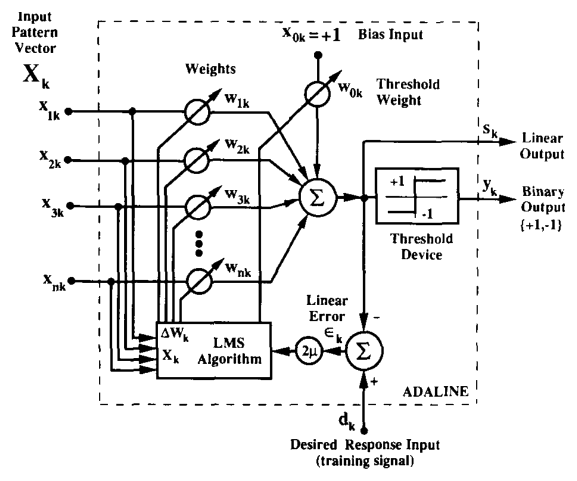
\includegraphics[width=\textwidth,height=0.66\textheight,keepaspectratio]{figuras/paper_adaline.png}\\
  {\scriptsize Fig.~2 del artículo: Adaline (combinador + cuantizador).}
\end{center}
\column{0.4\textwidth}
\begin{block}{Ecuaciones}
Producto interno: \[ s_k = X_k^{T} W_k \]
Cuantizador duro: $y_k = \operatorname{sgn}(s_k) \in \{\pm 1\}$.\\[2pt]
Variante diferenciable: $y_k = \tanh(s_k)$.
\end{block}
\begin{tipbox}
El bias $w_0$ ($+1$) fija el umbral; $s=0$ define el \textbf{hiperplano separador}.
\end{tipbox}
\end{columns}
\end{frame}

\begin{frame}{Separabilidad lineal y capacidad de patrones}
\begin{columns}[T]
\column{0.47\textwidth}
\begin{center}
  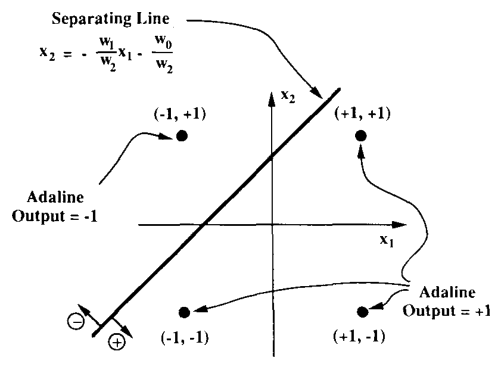
\includegraphics[height=4.3cm, keepaspectratio]{figuras/paper_frontera_lineal.png}\\
  {\scriptsize Fig.~4: $s=0$ como recta separadora. Ninguna recta separa \azul{XOR}.}
\end{center}
\column{0.5\textwidth}
\begin{block}{Límite del Adaline}
Con $n=2$ entradas implementa \textbf{14 de 16} funciones lógicas; imposibles: \azul{XOR} y \azul{XNOR}
(no separables) $\Rightarrow$ exigen \azul{no linealidad}.
\end{block}
\begin{itemize}\footnotesize
  \item Capacidad determinística: $C_d = N_w$ (garantía).
  \item Capacidad estadística (Cover): $\azul{C_s \approx 2N_w}$ (promedio); Baum la extendió a redes.
  \item No realizar \emph{todas} las funciones \textbf{limita la capacidad y mejora la generalización}.
\end{itemize}
\end{columns}
\end{frame}

\begin{frame}{De Madaline~I a la red multicapa: el problema de las capas ocultas}
\vspace{-15pt}
\begin{columns}[T]
\column{0.5\textwidth}
\begin{center}
  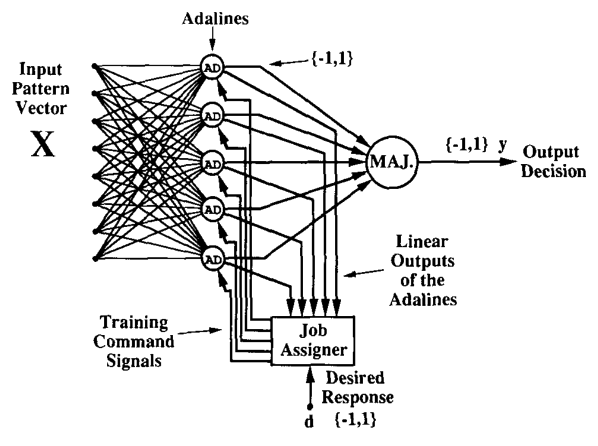
\includegraphics[width=\textwidth,height=0.46\textheight,keepaspectratio]{figuras/paper_madaline1.png}\\
  {\scriptsize Fig.~15: Madaline~I - Adalines \emph{signum} + \azul{lógica fija} (solo 1.\textsuperscript{a} capa adaptativa).}
\end{center}
\column{0.5\textwidth}
\begin{center}
  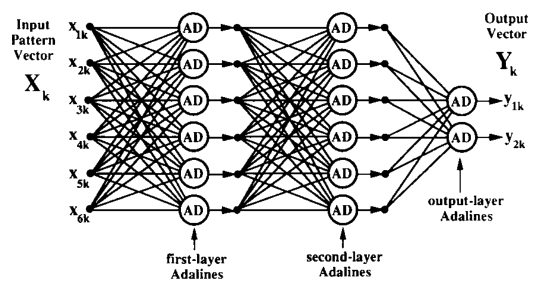
\includegraphics[width=\textwidth,height=0.42\textheight,keepaspectratio]{figuras/paper_red_3capas.png}\\
  {\scriptsize Fig.~11: red \emph{feedforward} moderna - \azul{todas} las capas adaptativas.}
\end{center}
\end{columns}
\begin{ideaclave}\footnotesize
La dificultad clave es obtener \azul{señales de error} para las capas \textbf{ocultas}.
\emph{Backpropagation} y \emph{Madaline Rule III} son precisamente los dos mecanismos que la resuelven.
\end{ideaclave}
\end{frame}

% =====================================================================
\section{Reglas de aprendizaje}
% =====================================================================
\subsection{Corrección de error y descenso de gradiente}

\begin{frame}{Dos familias de reglas y su taxonomía (Fig.~33)}
\begin{columns}[T]
\column{0.36\textwidth}
\begin{block}{Corrección de error}\footnotesize
Corrigen una \azul{proporción del error} en el patrón presente (\emph{ad hoc}, útil con no linealidades duras).
\end{block}
\begin{block}{Descenso más pronunciado}\footnotesize
Minimizan el \azul{MSE promediado} por gradiente sobre todo el conjunto.
\end{block}
\column{0.62\textwidth}
\begin{center}
\resizebox{\textwidth}{!}{%
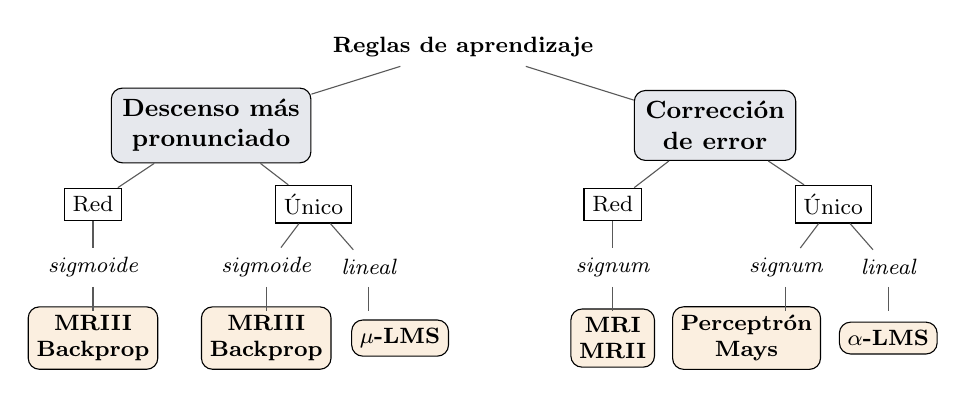
\begin{tikzpicture}[every node/.style={font=\footnotesize}]
  \node (root) at (0,4.2) {\textbf{Reglas de aprendizaje}};
  \node[cat] (sd) at (-3.2,3.2) {Descenso más\\pronunciado};
  \node[cat] (ec) at (3.2,3.2) {Corrección\\de error};
  \draw[ln] (root)--(sd); \draw[ln] (root)--(ec);
  \node[arch] (sdL) at (-4.7,2.2) {Red};
  \node[arch] (sdS) at (-1.9,2.2) {Único};
  \node[arch] (ecL) at (1.9,2.2) {Red};
  \node[arch] (ecS) at (4.7,2.2) {Único};
  \draw[ln] (sd)--(sdL);\draw[ln] (sd)--(sdS);\draw[ln] (ec)--(ecL);\draw[ln] (ec)--(ecS);
  \node[act] (a1) at (-4.7,1.4) {sigmoide};
  \node[act] (a2) at (-2.5,1.4) {sigmoide};
  \node[act] (a3) at (-1.2,1.4) {lineal};
  \node[act] (a4) at (1.9,1.4) {signum};
  \node[act] (a5) at (4.1,1.4) {signum};
  \node[act] (a6) at (5.4,1.4) {lineal};
  \draw[ln] (sdL)--(a1);\draw[ln] (sdS)--(a2);\draw[ln] (sdS)--(a3);
  \draw[ln] (ecL)--(a4);\draw[ln] (ecS)--(a5);\draw[ln] (ecS)--(a6);
  \node[alg] at (-4.7,0.5) {MRIII\\Backprop};
  \node[alg] at (-2.5,0.5) {MRIII\\Backprop};
  \node[alg] at (-0.8,0.5) {$\mu$-LMS};
  \node[alg] at (1.9,0.5) {MRI\\MRII};
  \node[alg] at (3.6,0.5) {Perceptr\'on\\Mays};
  \node[alg] at (5.4,0.5) {$\alpha$-LMS};
  \foreach \x in {-4.7,-2.5,-1.2,1.9,4.1,5.4}{\draw[ln] (\x,1.15)--(\x,0.85);}
\end{tikzpicture}}

{\scriptsize Reproducción fiel de la Fig.~33 del artículo.}
\end{center}
\end{columns}
\end{frame}

\begin{frame}{Corrección de error de un elemento: $\alpha$-LMS y Perceptrón}
\begin{columns}[T]
\column{0.5\textwidth}
\begin{block}{$\alpha$-LMS (Widrow-Hoff, lineal)}
\[ W_{k+1}=W_k+\alpha\,\frac{\varepsilon_k}{\lVert X_k\rVert^{2}}X_k,\;\; \varepsilon_k=d_k-X_k^{T}W_k \]
\footnotesize Corrección $\propto$ error \azul{lineal}; auto-normalizante; $0<\alpha<2$.
\end{block}
\column{0.5\textwidth}
\begin{block}{Perceptrón (Rosenblatt, no lineal)}
\[ W_{k+1}=W_k+\alpha\,\frac{\tilde{\varepsilon}_k}{2}X_k,\;\; \tilde{\varepsilon}_k=d_k-y_k \]
\footnotesize Usa el error del \azul{cuantizador}; solo adapta si $y_k\neq d_k$.
\end{block}
\end{columns}
\begin{itemize}\footnotesize
  \item \naranja{Perceptrón}: converge en pasos finitos \textbf{si} los datos son separables; si no, oscila y el peso ``gravita a cero''.
  \item \naranja{$\alpha$-LMS}: estable siempre, pero su objetivo es reducir el error lineal, no \emph{separar}.
  \item \emph{Reglas de Mays}: introducen una \azul{zona muerta} $\gamma$; con datos no separables suelen superar al Perceptrón.
\end{itemize}
\end{frame}

\begin{frame}{Corrección de error multicapa: Madaline Rule II (Fig.~16)}
\begin{columns}[T]
\column{0.5\textwidth}
\begin{center}
  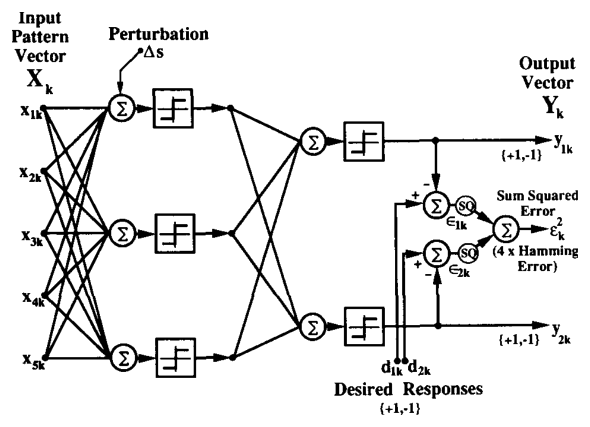
\includegraphics[width=\textwidth,height=0.6\textheight,keepaspectratio]{figuras/paper_mrii.png}
\end{center}
\column{0.5\textwidth}
\begin{block}{MRII (Widrow, Winter \& Baxter, 1987)}\footnotesize
Ambas capas adaptativas. Por cada patrón erróneo:
\begin{enumerate}
  \item Ordenar Adalines por $|s|$ (mínima perturbación).
  \item \azul{Flip tentativo}: si reduce el \textbf{error de Hamming}, se acepta y se refuerza con $\alpha$-LMS.
  \item Si no, probar \emph{pares}; capa de salida por $\alpha$-LMS.
\end{enumerate}
\end{block}
\begin{alertblock}{Limitación}\footnotesize
Cuantizadores duros $\Rightarrow$ \textbf{óptimos locales}. Remedio: ruido esporádico o \emph{random restarts}.
\end{alertblock}
\end{columns}
\end{frame}

\begin{frame}{Descenso de gradiente lineal: $\mu$-LMS y la superficie de MSE}
\begin{columns}[T]
\column{0.52\textwidth}
\begin{block}{Regla $\mu$-LMS}
\[ W_{k+1}=W_k+2\mu\,\varepsilon_k\,X_k \]
Superficie de MSE (paraboloide \azul{convexo}):
\[ \xi(W)=\mathbb{E}[d^2]-2P^{T}W+W^{T}RW \]
Mínimo único (solución de Wiener): $\;W^{*}=R^{-1}P$.
\end{block}
\column{0.46\textwidth}
\begin{center}
  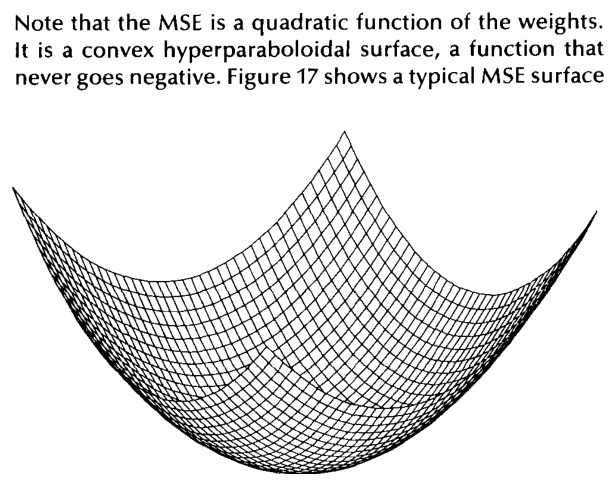
\includegraphics[width=\textwidth,height=0.42\textheight,keepaspectratio]{figuras/paper_mse_bowl.png}\\
  {\scriptsize Fig.~17: MSE del combinador lineal.}
\end{center}
\begin{itemize}\footnotesize
  \item Gradiente instantáneo $-2\varepsilon_k X_k$: estimador \azul{insesgado}.
  \item $\mu$-LMS $\to$ mínimo MSE (Wiener); $\alpha$-LMS, a solución sesgada.
\end{itemize}
\end{columns}
\end{frame}

\begin{frame}{Por qué el gradiente exige activaciones diferenciables (Figs.~22--24)}
\begin{center}
  
\includegraphics[width=0.9\textwidth, keepaspectratio]{figuras/fig_superficies_mse.png}
\end{center}
\vspace{-2pt}\footnotesize
\begin{columns}[T]
\column{0.32\textwidth}
\begin{tipbox}\textbf{Lineal}: paraboloide convexo, mínimo global garantizado.\end{tipbox}
\column{0.32\textwidth}
\begin{tipbox}\textbf{Sigmoide}: suave y navegable; posibles mínimos locales.\end{tipbox}
\column{0.32\textwidth}
\begin{alertblock}{Signum}\textbf{Mesetas} de gradiente nulo: el descenso se detiene.\end{alertblock}
\end{columns}
\end{frame}

\begin{frame}{Descenso de gradiente no lineal: Backpropagation (Fig.~25)}
\begin{columns}[T]
\column{0.52\textwidth}
\begin{center}
  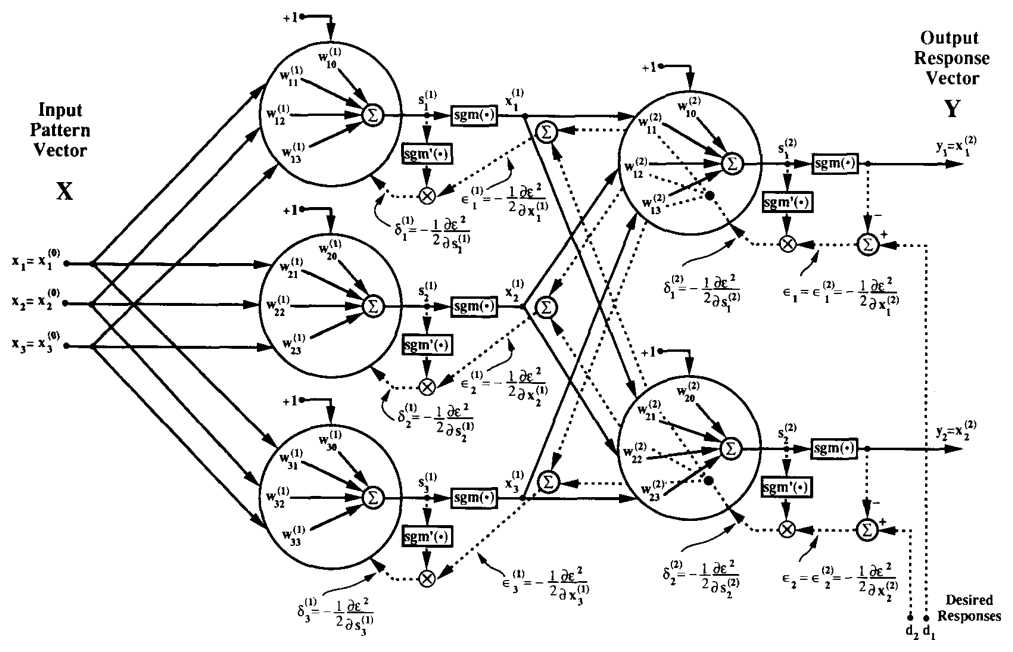
\includegraphics[width=\textwidth,height=0.6\textheight,keepaspectratio]{figuras/paper_bp_red.png}\\
  {\scriptsize Trazo continuo = ida ($X\to Y$); punteado = retorno de los $\delta$.}
\end{center}
\column{0.46\textwidth}
\begin{block}{Propagación del error}\footnotesize
Salida y capas ocultas:
\[ \delta^{(L)}_j=\varepsilon_j(1-y_j^{2}) \]
\[ \delta^{(l)}=\big(W^{(l+1)T}\delta^{(l+1)}\big)\odot(1-(y^{(l)})^{2}) \]
Update ($+$ momentum $\eta\!\approx\!0.9$): $\Delta W_k=2\mu\,\delta_k X_k^{T}$.
\end{block}
\begin{ideaclave}\footnotesize
$\delta$ \textbf{no es un error}: es una \azul{señal de gradiente} para reducir $\varepsilon^2$ de salida.
\end{ideaclave}
\end{columns}
\end{frame}

\begin{frame}{Madaline Rule III $\equiv$ Backpropagation (Fig.~28)}
\begin{columns}[T]
\column{0.5\textwidth}
\begin{center}
  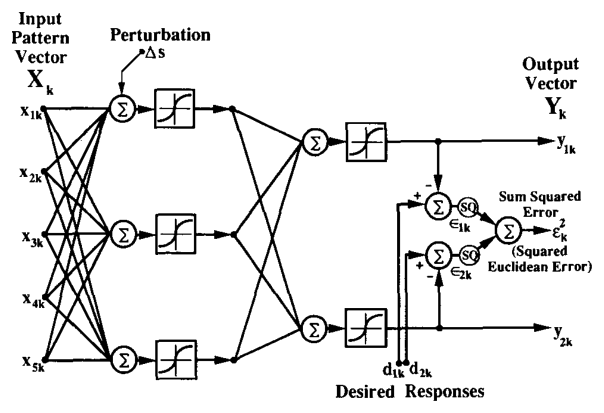
\includegraphics[width=\textwidth,height=0.5\textheight,keepaspectratio]{figuras/paper_mriii_red.png}\\
  {\scriptsize Misma arquitectura que MRII, pero con \azul{sigmoides}.}
\end{center}
\column{0.5\textwidth}
\begin{block}{MRIII (Andes, 1988)}\footnotesize
Gradiente por \azul{perturbación} del sumidero, sin la derivada de la sigmoide:
\[ \frac{\partial \varepsilon^2}{\partial s_j}\approx\frac{\varepsilon^2_{\text{pert}}-\varepsilon^2_{\text{base}}}{\Delta s} \]
\end{block}
\begin{ideaclave}\footnotesize
Con $\Delta s\to 0$, MRIII es \textbf{matemáticamente equivalente a backpropagation}; \azul{robusto} en
hardware analógico (existió un chip comercial).
\end{ideaclave}
\end{columns}
\end{frame}

% =====================================================================
\section{Experimentos}
% =====================================================================
\subsection{Diseño y resultados}

\begin{frame}{Diseño experimental: hipótesis y mapa}
\begin{block}{Objetivo}\footnotesize
Validar \textbf{numéricamente} las afirmaciones del artículo. Todo implementado \azul{desde cero en NumPy}
(\emph{scikit-learn} solo para cargar datos y métricas). Datos: sintéticos (separable, no separable, XOR)
y reales (Iris, Wine, MNIST-04, two-moons).
\end{block}
{\footnotesize
\renewcommand{\arraystretch}{1.25}
\begin{tabular}{@{}c p{0.86\textwidth}@{}}
\toprule
\textbf{Hip.} & \textbf{Descripción} \\
\midrule
\azul{H1} & Un Adaline de $N_w$ pesos almacena en promedio $C_s\approx 2N_w$ patrones ($C_d=N_w$ garantizado). \\
\azul{H2} & El Perceptrón converge solo si hay separabilidad; $\alpha$/$\mu$-LMS estables, con $\mu$-LMS $\to$ Wiener $R^{-1}P$. \\
\azul{H3} & Los problemas no separables (XOR) exigen multicapa; la superficie sigmoide es más navegable que la signum. \\
\azul{H4} & El gradiente de MRIII (perturbación) coincide con el de backprop cuando $\Delta s\to 0$. \\
\bottomrule
\end{tabular}}
\end{frame}

\begin{frame}{E1 --- Capacidad de Cover (H1)}
\begin{columns}[T]
\column{0.5\textwidth}
\begin{center}
  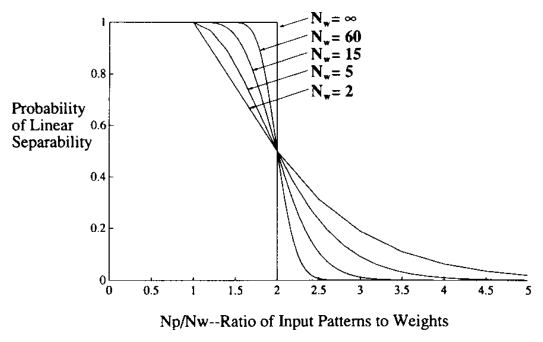
\includegraphics[width=\textwidth,height=0.44\textheight,keepaspectratio]{figuras/paper_cover.png}\\
  {\scriptsize Fig.~5 del artículo (teoría, 1965).}
\end{center}
\column{0.5\textwidth}
\begin{center}
  
\includegraphics[width=\textwidth,height=0.44\textheight,keepaspectratio]{figuras/fig_cover.png}\\
  {\scriptsize Reconstrucción empírica (Monte Carlo).}
\end{center}
\end{columns}
\begin{ideaclave}\footnotesize
\textbf{H1 confirmada}: desviación media $\leq 0.034$ entre empírico y teoría. Se verifica $C_d=N_w$
(en $N_p/N_w=1$) y $C_s\approx 2N_w$ (probabilidad $0.5$).
\end{ideaclave}
\end{frame}

\begin{frame}{E2--E3 --- Reglas lineales \emph{vs.} óptimo de Wiener (H2)}
\begin{center}
  
\includegraphics[width=\textwidth,height=0.5\textheight,keepaspectratio]{figuras/fig_fronteras.png}\\
  {\scriptsize Fronteras aprendidas por cada regla \emph{vs.} Wiener (datos separables).}
\end{center}
\begin{ideaclave}\footnotesize
\textbf{H2 confirmada}. \azul{Separable}: el Perceptrón converge (2 épocas) pero queda a $20.6^\circ$ de
Wiener; $\mu$-LMS a solo $3.5^\circ$. \azul{No separable}: el Perceptrón oscila; $\mu$-LMS es el mejor
($79.6\%$ \emph{vs.} Wiener $81.0\%$) y de menor varianza.
\end{ideaclave}
\end{frame}

\begin{frame}{E5 --- XOR: MRII \emph{vs.} MLP-Backpropagation (H3)}
\begin{columns}[T]
\column{0.58\textwidth}
\begin{center}
  
\includegraphics[width=\textwidth,height=0.55\textheight,keepaspectratio]{figuras/fig_xor.png}\\
  {\scriptsize \textbf{Datos: XOR} (4 patrones, no separable).}
\end{center}
\column{0.42\textwidth}
\renewcommand{\arraystretch}{1.15}
\begin{center}{\scriptsize
\begin{tabular}{@{}lc@{}}
\toprule
Configuración & Éxito \\
\midrule
MRII 2-2-1 & 0/20 \\
MRII 2-3-1 + ruido & 0/20 \\
MLP-BP 2-2-1 & 6/20 \\
MLP-BP 2-3-1 & 11/20 \\
\bottomrule
\end{tabular}}\end{center}
\begin{alertblock}{H3 confirmada}\footnotesize
Solo la multicapa resuelve XOR; MRII y backprop sufren óptimos locales.
\end{alertblock}
\end{columns}
\end{frame}

\begin{frame}{E6 --- Generalización a datos reales (H3)}
\begin{columns}[T]
\column{0.56\textwidth}
\begin{center}
  
\includegraphics[width=\textwidth,height=0.55\textheight,keepaspectratio]{figuras/fig_moons.png}\\
  {\scriptsize MLP-backprop sobre \textbf{two-moons}: frontera \azul{curva} imposible para un lineal.}
\end{center}
\column{0.44\textwidth}
\renewcommand{\arraystretch}{1.2}
\begin{center}{\footnotesize
\begin{tabular}{@{}lcc@{}}
\toprule
Dataset & Modelo & Test \\
\midrule
two-moons & MLP-BP & $93.3\%$ \\
Iris & MLP-BP & $91.1\%$ \\
Wine & $\mu$-LMS/Wiener & $98.1\%$ \\
MNIST-04 & MLP-BP & $98.5\%$ \\
\bottomrule
\end{tabular}}\end{center}
\begin{ideaclave}\footnotesize
\textbf{H3 confirmada}: la no linealidad generaliza a datos reales y \azul{escala} a mayor dimensión
(MNIST-04, 64 rasgos).
\end{ideaclave}
\end{columns}
\end{frame}

\begin{frame}{E7 --- Equivalencia MRIII $\equiv$ Backpropagation (H4)}
\begin{center}
  
\includegraphics[width=\textwidth,height=0.5\textheight,keepaspectratio]{figuras/fig_mriii_bp.png}\\
  {\scriptsize Gradiente de MRIII (perturbación) \emph{vs.} el analítico de backprop, y su costo.}
\end{center}
\begin{ideaclave}\footnotesize
\textbf{H4 confirmada}: el gradiente de MRIII converge al de backprop con error relativo mínimo de
$\azul{5.05\times10^{-8}}$; el costo crece como $\mathcal{O}(N_{\text{Adalines}})$.
\end{ideaclave}
\end{frame}

% =====================================================================
\section{Conclusiones}
% =====================================================================
\subsection{Síntesis}

\begin{frame}{Conclusiones}
\begin{block}{Aporte del artículo}
\begin{itemize}\footnotesize
  \item \textbf{Unifica 30 años} de algoritmos bajo un principio común: la \azul{mínima perturbación}.
  \item El linaje Perceptrón $\to$ Adaline $\to$ Madaline $\to$ Backprop es una \textbf{progresión lógica}.
  \item La equivalencia \azul{MRIII $\equiv$ backprop} muestra que un mismo descubrimiento llega por caminos independientes.
\end{itemize}
\end{block}
\begin{alertblock}{Evaluación de hipótesis}\footnotesize
\textbf{H1--H4 confirmadas}. Matiz en H3: MRII resultó más frágil ante óptimos locales que el MLP
($0/20$ con semilla única), tal como el propio artículo anticipa.
\end{alertblock}
\end{frame}

% ─── CIERRE ──────────────────────────────────────────────────────────
\begin{frame}[plain]
\vfill
\begin{center}
{\Huge\bfseries\azul{Gracias}}\\[10pt]
\footnotesize
30 Years of Adaptive Neural Networks: Perceptron, Madaline, and Backpropagation\\
\emph{B.\ Widrow \& M.\ A.\ Lehr}, Proceedings of the IEEE, 78(9), 1990.
\end{center}
\vfill
\end{frame}

\end{document}
